
\documentclass[letterpaper, 10 pt, conference]{ieeeconf}  
\IEEEoverridecommandlockouts                             
\usepackage{graphicx} 
\usepackage{hyperref}

\overrideIEEEmargins

\title{\Huge Image Mosaicing}
\author{Jiyu Tian} 

\begin{document}

\maketitle
\thispagestyle{empty}
\pagestyle{empty}

%-------------------------------------------------------------------------

\section{INTRODUCTION}
In this project we implement a technique for image mosaicing with feature matching. 
Harris corner detector is applied to find corners in two images. With corresponding features, a homography between the two images can then be estimated. Finally we warp one image into the coordinate system of the second one to produce a mosaic containing the union of all pixels in the two images.
%-------------------------------------------------------------------------
\section{ALGORITHMS DESCRIPTION}
\subsection{Grayscale Conversion}
After reading in two images, we first make them grayscale.We apply the conversion as the following eqaution:
\begin{equation}
Gray = 0.299 \times R + 0.587 \times G + 0.114 \times B
\end{equation}

If, in the worst case, input images do not have all the three $RGB$ channels, we simply regard the first channel as its grayscale value.
\subsection{Harris Corner Detector}
The image gradient $I_x$ and $I_y$ is computed using horizontal and vertical components of Prewitt/Sobel mask. Then at each pixel we compute products of derivatives $I^2_x$, $I^2_y$ and $I^2_{xy}$. A window centering at the pixel is selected for averaging the sums of the products $S^2_x$, $S^2_y$ and $S^2_{xy}$.
At each pixel, a matrix $M$ is defined as 
\begin{equation}
M=\left[ \begin{array}{cc}
S^2_x & S^2_{xy}\\
S^2_{xy} & S^2_y
\end{array} \right]
\end{equation}

And the response $R$ can be computed as
\begin{equation}
R=det(M) - k\times trace(M)^2
\end{equation}

\subsection{Correspondences}
Given two set of corners from the two images, we compute normalized cross correlation ($NCC$) of image patches centered at each corner. 
\begin{equation}
N_{fg} = \sum_{[i, j]\in R}\hat{f}(i, j)\hat{g}(i, j),\ \ \hat{f} = \frac{f}{||f||}, \ \  \hat{g} = \frac{g}{||g||}
\end{equation}

We choose potential corner matches by finding pair of corners (one from each image) such that they have the highest $NCC$ value. We also set a threshold to keep only matches pairs that have a large $NCC$ score.
\subsection{Homography Estimation}
Given a set of 4 points pairs $(x,y)\ (x', y')$, we can compute the homography from
\begin{equation}
\left[ \begin{array}{c}
x'\\
y'\\
1
\end{array} \right] = \left[ \begin{array}{ccc}
h_{11} & h_{12} & h_{13} \\
h_{21} & h_{22} & h_{23} \\
h_{31} & h_{32} & h_{33} 
\end{array} \right]\left[ \begin{array}{c}
x\\
y\\
1
\end{array} \right] 
\end{equation}

We use RANSAC to robustly estimate the homography from the noisy correspondences:
\begin{itemize}
\item Repeatedly sample 4 random points
\item Compute a homography from these four points
\item Map all points using the homagraphy and comparing distances between predicted and observed locations to determine the number of inliers
\item At the end, compute a least-squares homgraphy from \textbf{all} the inliers in the largest set of inliers.
\end{itemize}


\subsection{Image Warp}
After generating the homography, we can warp one image onto the other one, blending overlapping pixels together to create a single image that shows the union of all pixels from both input images. 

The steps are as follows:
\begin{itemize}
    \item Determine how big to make the final output image so that it contains the union of all pixels in the two images
    \item Copy the image that does not have to be warped into the appropriate location in the output
    \item Warp the other image into the output image based on the estimated homography
    \item Blend pixels in the area of overlap between both images
\end{itemize}
%-------------------------------------------------------------------------
\section{EXPERIMENTAL RESULTS}
The two raw images we adopt for report are shown in Fig \ref{raw}. They are converted into grayscale for the following steps. Please refer to the Appendix A for a complete flowchart.
\begin{figure}[thpb]
\centering
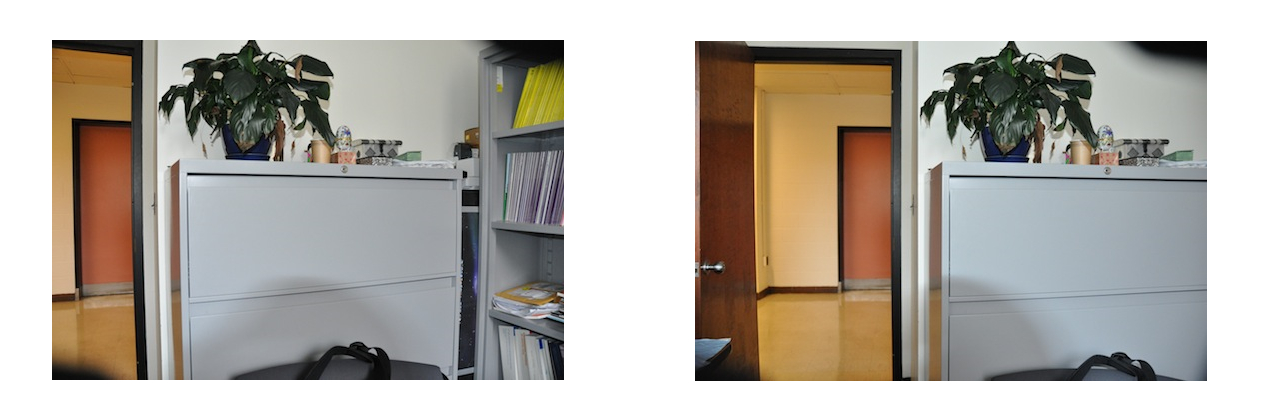
\includegraphics[width=0.5\textwidth]{raw.png}
\caption{Raw Images}
\label{raw}
\end{figure}
%--------------------------------------
\subsection{Corner Detection}
After applied by Harris corner detector, the corner features within two images are shown in Fig \ref{corner}.

The gradient is computed with Sobel mask. We utilize a $7\times7$ Gaussian averaging window with $\sigma=1.4$ to find matrix $M$ at each pixel. A threshold of $R = 1\times 10^8$ is set to filtered pixels with low response, and $k$ is set to $0.05$.

\begin{figure}[thpb]
\centering
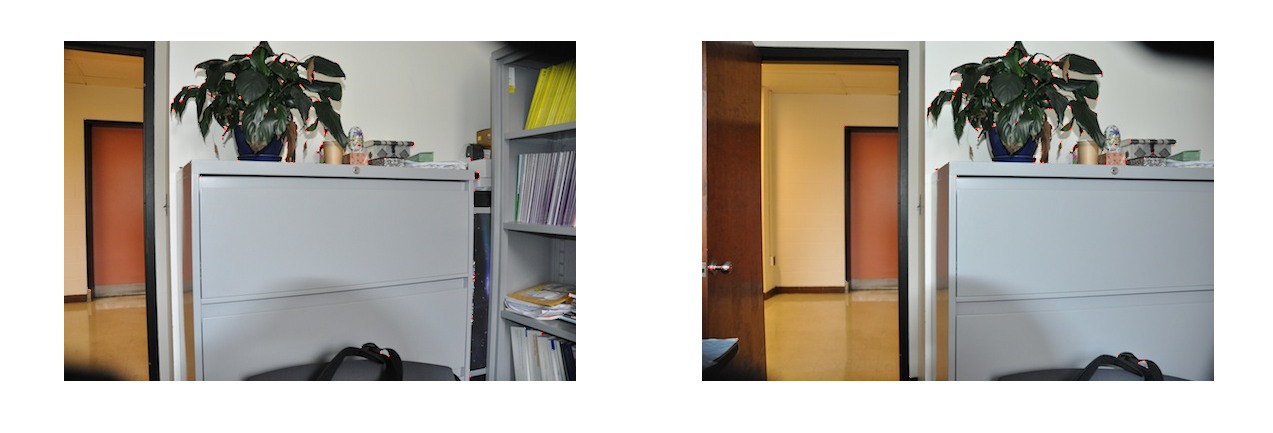
\includegraphics[width=0.5\textwidth]{corner.png}
\caption{Corner Detection Result}
\label{corner}
\end{figure}

We compute non-maximum suppression to find local peaks within $3\times3$ neighbors.

%--------------------------------------
\subsection{Correspondences}
For each pair of corners from two images, we compute their $NCC$ in a $3\time3$ window. We find the potential corner pairs from the highest to the lowest $NCC$ score larger than $0.5$.

The corresponding pairs with outliers are shown in Fig \ref{corr}. There are over $100$ pairs in total.

\begin{figure}[thpb]
\centering
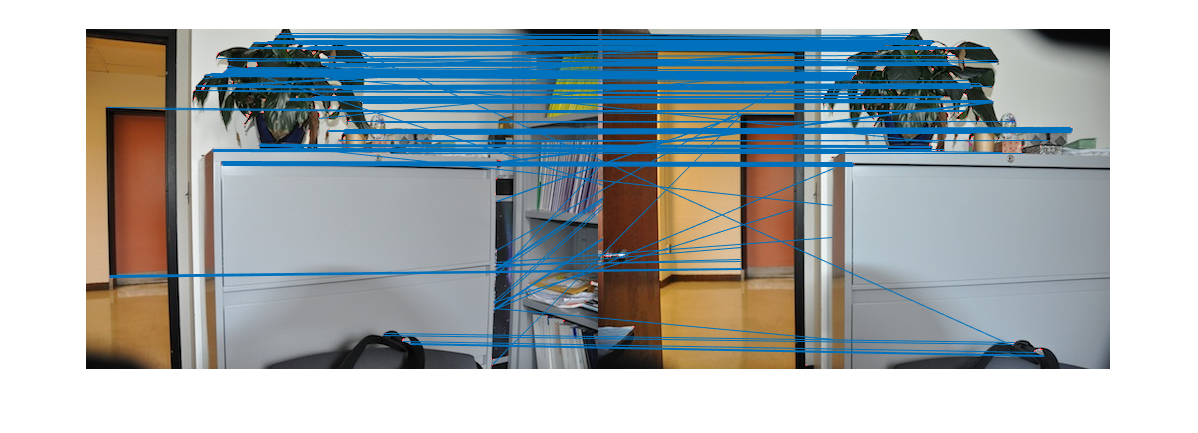
\includegraphics[width=0.5\textwidth]{correspondence.png}
\caption{Corresponding Pairs with Outliers}
\label{corr}
\end{figure}


%--------------------------------------
\subsection{Homography Estimation}
We run RANSAC to find final point correspondences. A total of $1\times10^4$ iterations are executed. A projected point is considered to be inlier if its Euclidien distance from matched point is less than $2$.

In a iteration, if $10\%$ of total points pairs are inliers, this
\newpage
\noindent homography is good enough; or a new set of four random point pairs is selected to compute homography.


\begin{figure}[thpb]
\centering
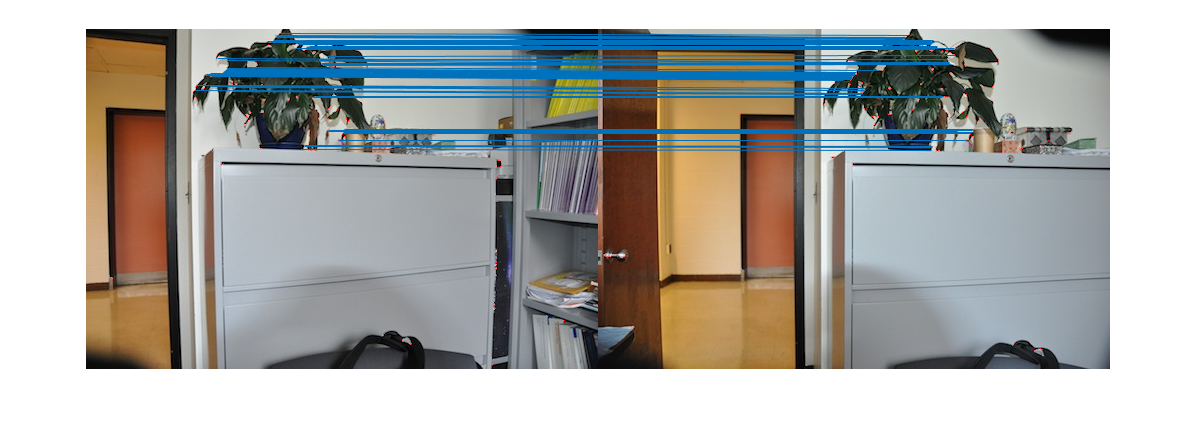
\includegraphics[width=0.5\textwidth]{ransac.png}
\caption{Cleaned Corresponding Pairs}
\label{clean}
\end{figure}

%--------------------------------------
\subsection{Final Mosaic}
As shown in Fig \ref{mosaic}, image $1$ is wrapped into image 2 with homography computed. In this part we utilize OpenCV for implementation.

\begin{figure}[thpb]
\centering
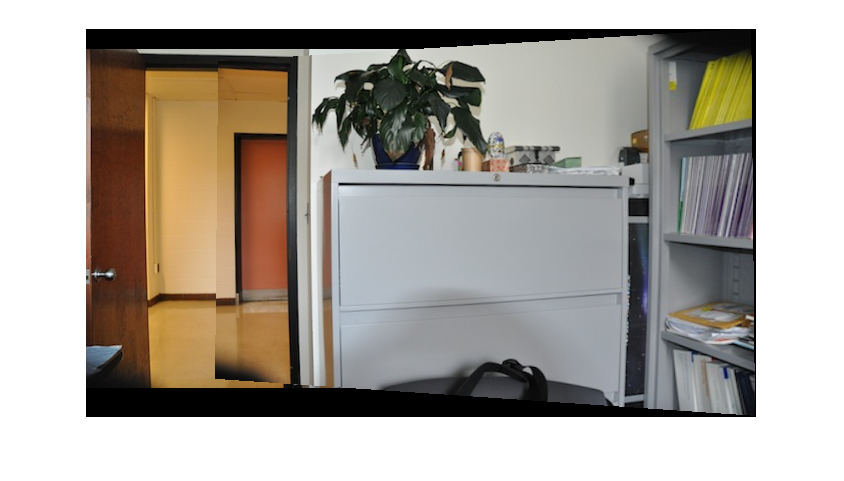
\includegraphics[width=0.4\textwidth]{mosaic.png}
\caption{Final Mosaic}
\label{mosaic}
\end{figure}

%--------------------------------------
\subsection{Limitation}
One key limitation of our algorithm is its high computing consumption. Plenty of time is spent on corner detection and correspondences computing, since the are $O(n^2)$ complexity.

We also notice that RANSAC process depends on the initial selection of point pairs. If luckily enough, iteration time can be reduced significantly.

%-------------------------------------------------------------------------
\section{CONCLUSION}
In this project, we explored various application of feature matching, and creatively applied them to image mosaicing. This is a very useful technique for constructing panoramic image mosaics from sequences of images.
\vfill

\end{document}
